\section{Overview}
\label{colors:overview}

% <The story goes:>
% 1. Connect motivation (from intro) to egg (as described in background), highlight uses in TheSy (and ruler)
% 2. General concept of colored (layered) e-classes
%    2.a. Explain clone semantics and how colored e-classes are equivalent
% 3. What e-graph operations need to be modified to support colored e-classes
% 4. Challenges and problems (performance bottlenecks caused by the new design)
% 5. Summary of optimization (primer for next section)

\begin{figure}[t]
  \centering
\begin{comment}
  \node(black)[label={above:$\cong$},
               label={[sub]below:{\small (a)}}] {
  %$\cong$ & $\congblue$ & $\congred$ \\
    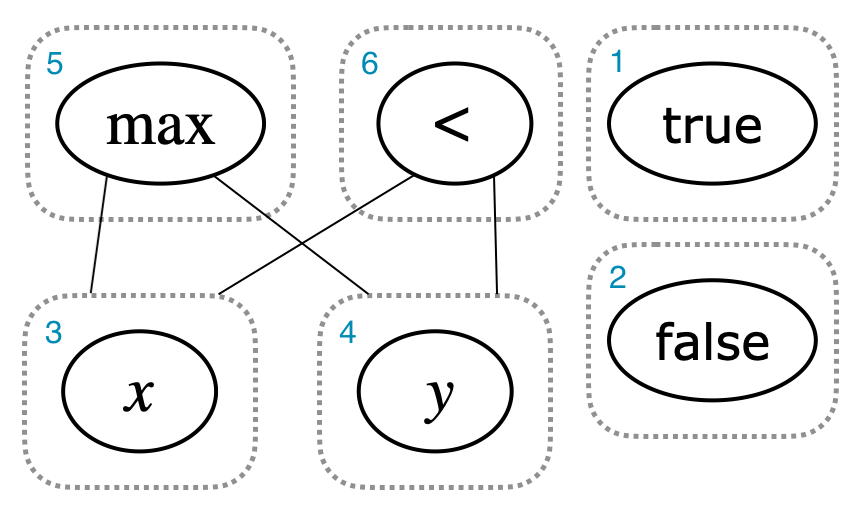
\includegraphics[width=2.7cm,valign=c]{gfx/egraph-max.png}
  };
\end{comment}

  \begin{tikzpicture}[sub/.style={label distance=0,outer sep=0,inner sep=0}]
  \node(blue) [label={[sub]above:$\congblue\!\!$},
               label={[sub]below:{\small (a)}}] {
    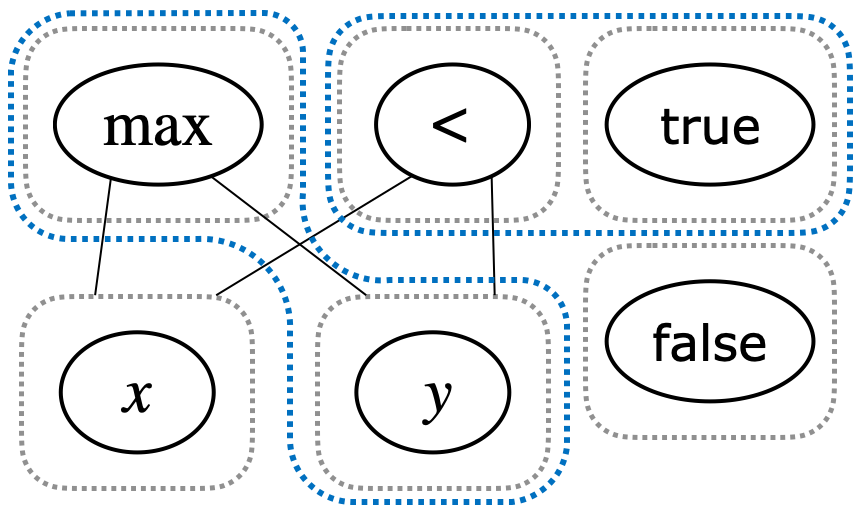
\includegraphics[width=2.7cm,valign=c]{colors/gfx/egraph-max-blue.png}    
  };
  \node(red)[right=0mm of blue,
             label={[sub]above:$\congred$},
             label={[sub]below:{\small (b)}}] {
    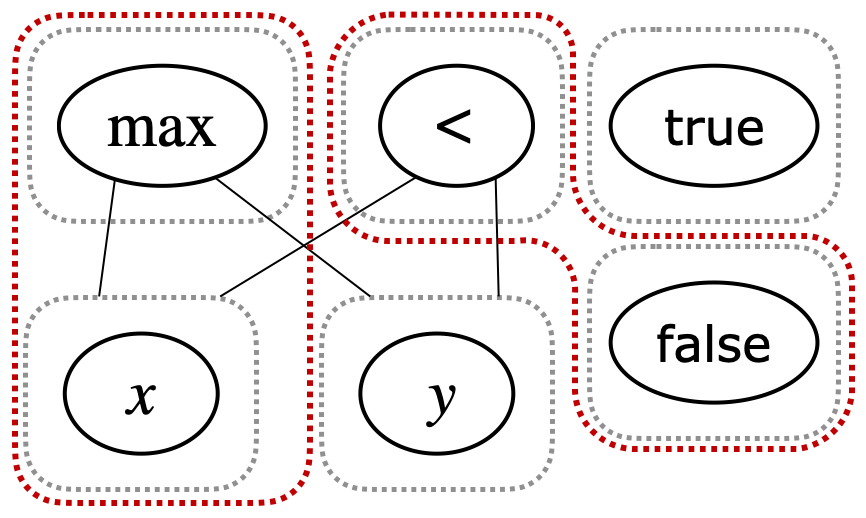
\includegraphics[width=2.7cm,valign=c]{colors/gfx/egraph-max-red.png}
  };
  \node(mixed)[right=0mm of red,
               label={[sub]below:{\small (c)}}] {
    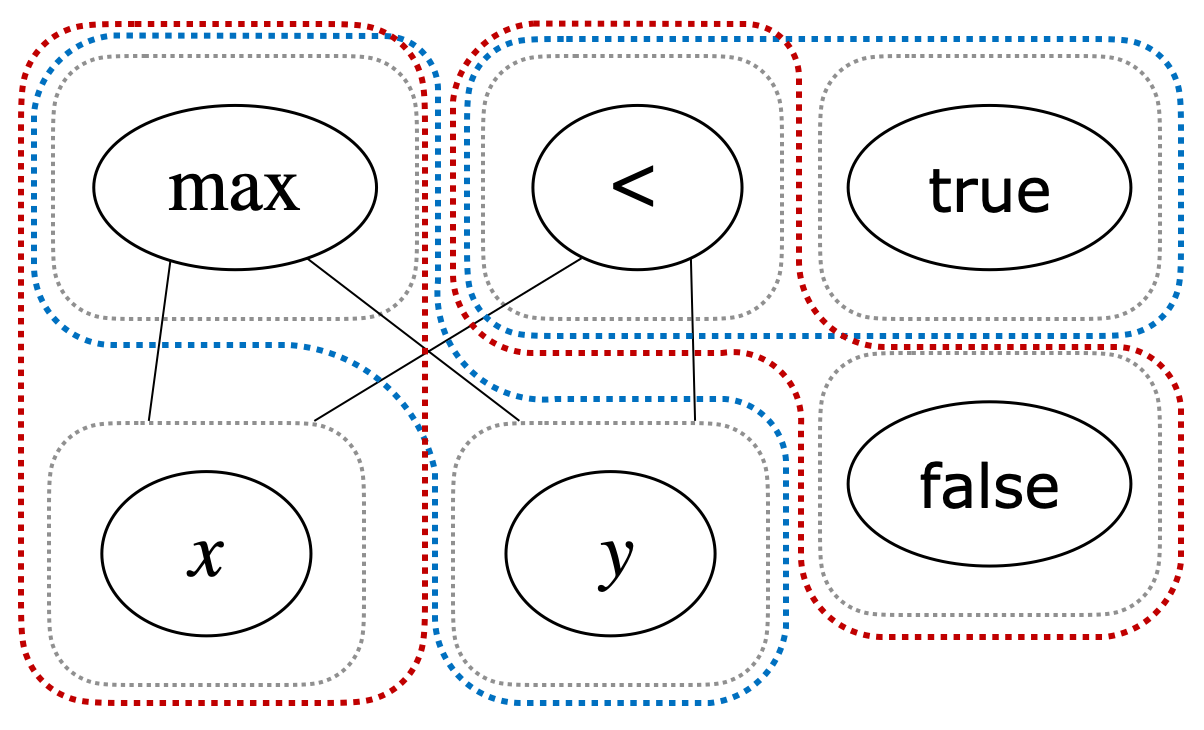
\includegraphics[width=2.9cm]{colors/gfx/egraph-max-red-blue.png}  
  };
  \end{tikzpicture}
  
  \caption[Example e-graph with two colored layers]{Example e-graph with two colored layers; (a) is blue, (b) is red, (c) shows them combined.}
  \label{overview:egraph-max}
\end{figure}

From this point we assume familiarity with the basic e-graph structure which includes a union-find, hashcons, and an e-class map, as well as the basic operations of add, merge, rebuild, and e-matching (and consequently rewriting).
For readers unfamiliar with e-graphs, or with deferred rebuilding, which was introduced in \cite{egg}, additional background is given in  \autoref{perlims:e-graphs}.

\emph{Colored E-graphs} are an extension of e-graphs devised to add a generic approach for supporting conditional reasoning to e-graphs.
Existing exploratory reasoning systems such as TheSy~\cite{thesy} and Ruler~\cite{ruler} utilize equality saturation with e-graphs for discovering new rewrite rules, but are limited in the presence of conditionals.
For example, let $t := \tmax(x, y)$, then reasoning about the cases $x < y$ and $x \geq y$ separately is desirable: in the first case $t \cong x$, and in the second $t \cong y$.
Without any assumptions, we can say neither and rewriting of $t$ is blocked.
The approach in \cite{thesy} involves a prover that creates an e-graph \emph{clone} for each case in case splitting, such as for $x < y$ and $x \geq y$. 
This process, however, incurs high runtime and memory costs. 
Non-relevant terms in the e-graph are unnecessarily duplicated, and rewrites are redundantly applied to these copies. 
Further case splits compound this issue, leading to an exponential increase in the number of clones with additional nested splits.

%\ES{represent colored e-graphs shortly because it was last seen in the intro}

Colored e-graphs are designed to avoid duplication via sharing of the common terms, thus storing them only once when possible.
The e-graph structure becomes \emph{layered}:
the lowermost layer represents a congruence relation over terms that is true in all cases (represented, normally, as e-classes containing e-nodes).
On top of it are layered additional congruence relations that arise from various assumptions.


Going back to our example, the corresponding e-graph is
shown in \autoref{overview:egraph-max},
containing the terms $\tmax(x, y)$, $x < y$, $\ttrue$ and $\tfalse$.
Layers corresponding to assumptions $x < y$ and $x \geq y$ are shown in \ref{overview:egraph-max}(a) and \ref{overview:egraph-max}(b).
To evoke intuition, we associate with each layer a unique \emph{color}, and paint their e-classes (dotted outlines, in depicted e-graphs) accordingly.
Conventionally, the lowermost layer is associated with the color black.
In the subsequent example we will use \cblue for $x<y$ and \cred for $x\geq y$ when referring to the example.
In the \cblue layer, $(x < y) \congblue \ttrue$ and
$\tmax(x, y) \congblue y$;
in the \cred layer, $(x < y) \congred \tfalse$
and $\tmax(x, y) \congred x$.
This is shown via the corresponding 
\cblue and \cred dotted borders.
\autoref{overview:egraph-max}(c) shows a depiction where both colors are overlain on the same graph, which is a more faithful representation of the concept of colored e-graphs,
although this visualization is clearly not scalable to larger graphs.
In \autoref{overview:egraph-max-min}, a larger graph can be seen that includes the terms $\tmax(x,y)-\tmin(x,y)$ and $|x-y|$.
An overlain graph will be quite incomprehensible in this case, so the layers are shown separately; it can be easily discerned that $\tmax(x,y)-\tmin(x,y) \congblue |x-y|$
as well as $\tmax(x,y)-\tmin(x,y) \congred |x-y|$.

\begin{figure*}[t]
  \centering
  \begin{tabular}{@{}ccc@{}}
    $\cong$ & $\congblue$ & $\congred$ \\
    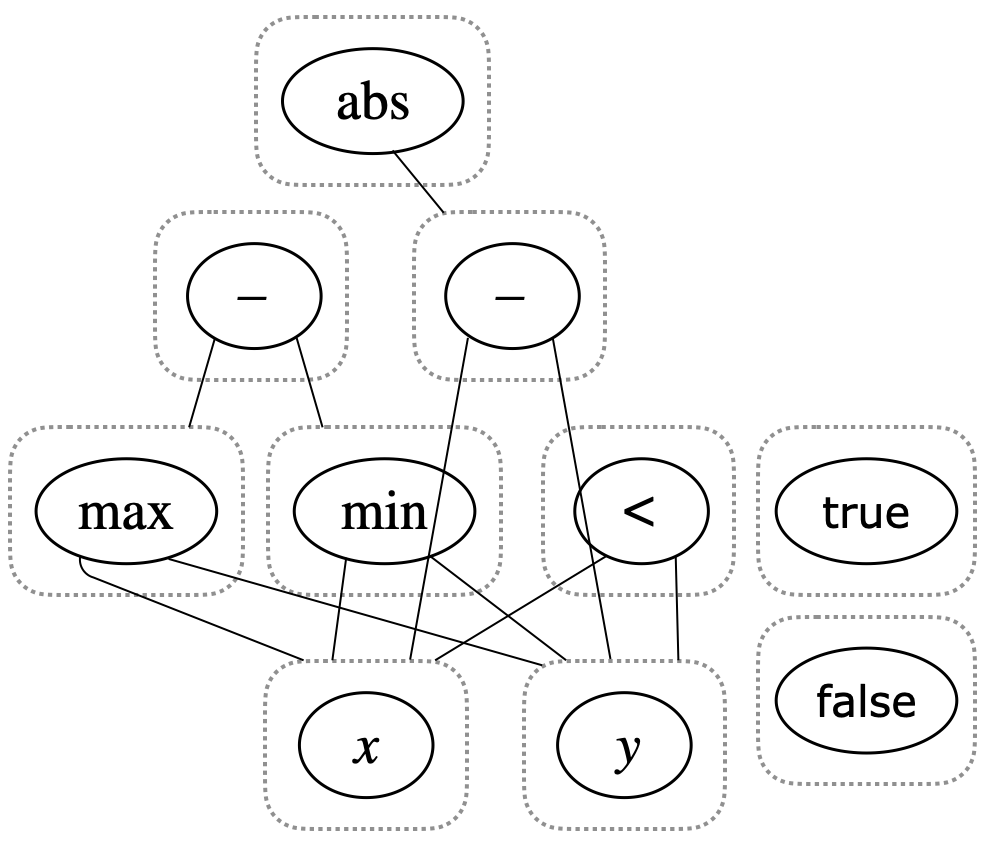
\includegraphics[width=0.25\textwidth]{colors/gfx/egraph-max-min.png} &
    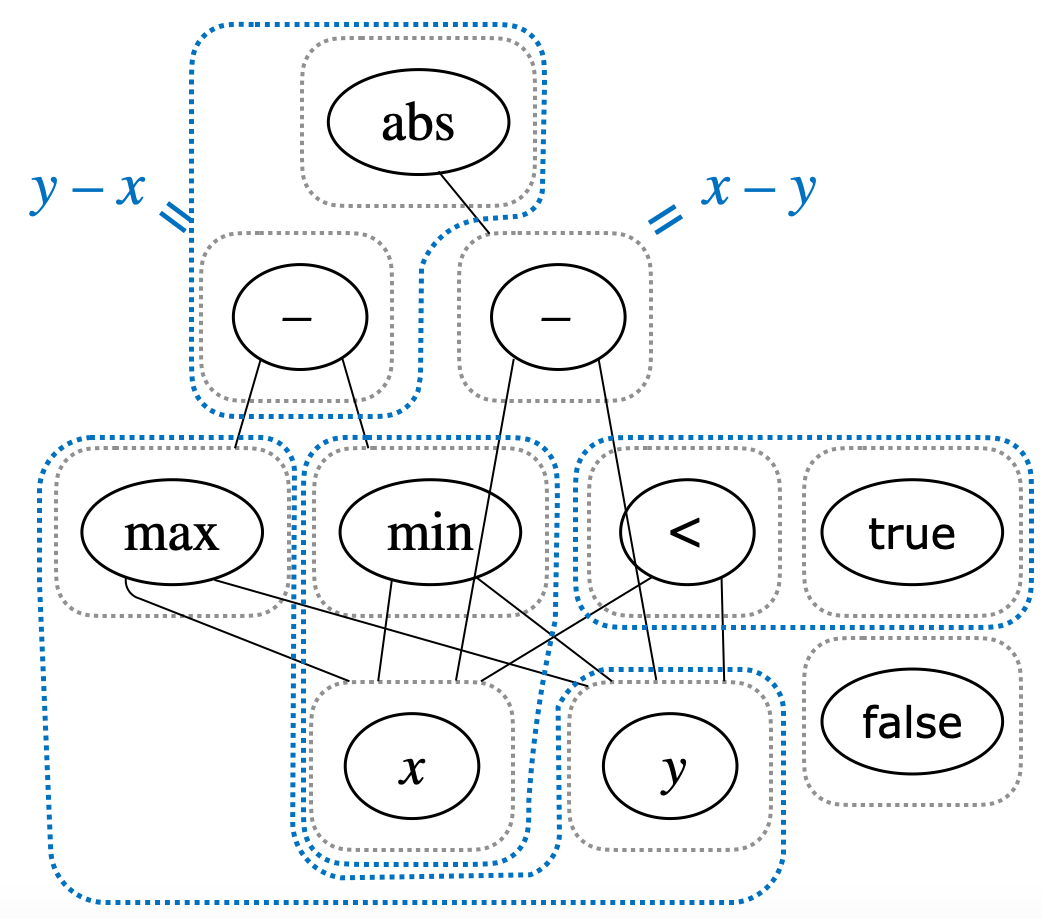
\includegraphics[width=0.25\textwidth]{colors/gfx/egraph-max-min-blue.png} &
    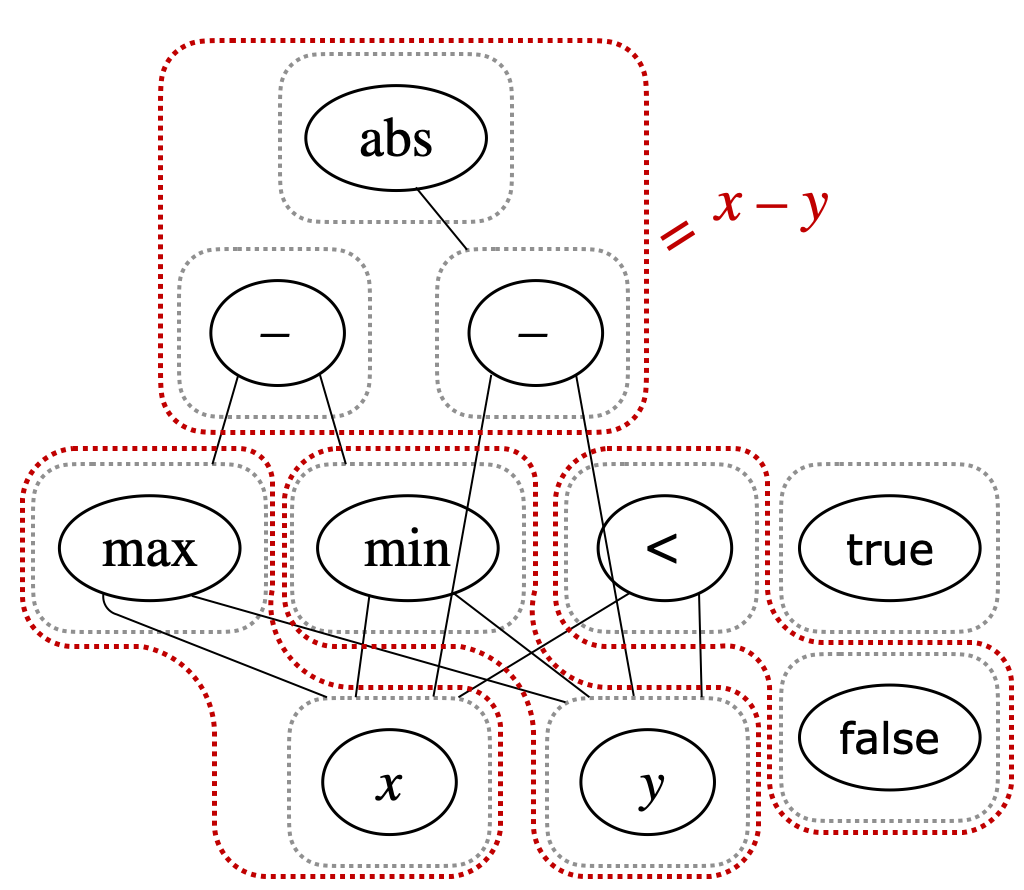
\includegraphics[width=0.25\textwidth]{colors/gfx/egraph-max-min-red.png}
    \\
    {\small (a)} & {\small (b)} & {\small (c)}
  \end{tabular}
  \caption[Proof of $\tsmallmax(x,y)-\tsmallmin(x,y)=|x-y|$]{Proof of $\tsmallmax(x,y)-\tsmallmin(x,y)=|x-y|$.
  The e-nodes corresponding to the two terms are in the same e-class both in the blue layer (b) and in the red (c).
   It is important to note that the layers are overlain, and that the black nodes are shared; they are separated here for ease of perception.}
  \label{overview:egraph-max-min}
\end{figure*}

Both additional layers, \cblue and \cred, use existing (black) e-nodes, with each color represented by further unions of e-classes in the black congruence relation. 
Each color's congruence $\cong_c$ is a \emph{coarsening} of the black congruence, $\cong$, as ${\cong}\subseteq{\cong_c}$.
% Hierarchy exmaple
In complex cases like the generalization of $\tmax(x,y)-\tmin(x,y) \cong |x-y|$ to $\tmax(x,y,z)-\tmin(x,y,z) \cong \tmax(|x-y|, |x-z|, |y-z|)$, the colored e-graphs have an important layered structure. 
This scenario requires reasoning about additional assumptions, building additional layers, such as $x < y \land y < z$ on top of $x < y$ (and respectively $x \ge y \land y < z$ on top of $x \ge y$). 
These additional layers will reuse the \cblue and \cred ones, as they are a coarsening of the respective $\congblue$ and $\congred$.

\begin{comment}
The extra colors are due to the conditionals from $\tmax$, $\tmin$, and $|\,{\cdot}\,|$ leading to a total of six leaf cases as can be seen in \autoref{overview:minmax-splits}.
The coarsening of congruence relation holds in this multi-level hierarchy as well.
If we mark in \cblue the layer representing $(x < y) \congblue \ttrue$, and in \cgreen the layer representing $x < y \land y < z \conggreen \ttrue$, then ${\congblue}\subseteq{\conggreen}$.
That is, any common sub-term and conclusion made in root, or one of the parent colors can be shared to the descendants.
Thus, further duplication, whether of terms or computation, can be prevented.
%Note, that this is not a full tree as in some cases we can conclude the $<$ relation between $x$ and $z$. 
%For example, in the case of $x < y \land y < z$ we can conclude $x < z$ without additional case splitting.

\begin{figure}
\begin{tikzpicture}[
    grow=down,
    level 1/.style={sibling distance=50mm, level distance=20mm},
    level 2/.style={sibling distance=25mm, level distance=20mm},
    level 3/.style={sibling distance=25mm, level distance=20mm},
    edge from parent/.style={->, draw},
    >=latex,
    every node/.style={align=center}]

% root of the tree
\node (root) {root}
% children of root
    child{node {$x < y$}
        % children of "x >= y"
        child{node {$x < y \land y \ge z$}
            child{node {$\cdots \land x < z$}}
            child{node {$\cdots \land x \ge z$}}
        }
        child{node {$x < y \land y < z$}}
    }
    child{node {$x \ge y$}
        % children of "x < y"
        child{node {$x \ge y \land y \ge z$}}
        child{node {$x \ge y \land y < z$}
            child{node {$\cdots \land x < z$}}
            child{node {$\cdots \land x \ge z$}}
        }
    };
\end{tikzpicture}
\caption{All needed case split cases to reason about the property $\tmax(x,y,z)-\tmin(x,y,z) \cong \tmax(|x-y|, |x-z|, |y-z|)$}
\label{overview:minmax-splits}
\end{figure}
\end{comment}

\begin{comment}
A crucial challenge to address is the implementation of operations (insert, union, congruence closure, e-matching)
efficiently while preserving this invariant as well as the standard e-graph invariants.
The colored layers require special support, as different e-classes may be united in some colored (non-black) layer but not in others (including the black relation). 
Notably, the black congruence relation can be implemented as a standard e-graph since all the necessary data structures are available to it.
\end{comment}

% Clone semantics
Before diving into the design of colored e-graphs, it is better to start with their expected semantics.
One way to understand the semantics of colored e-graphs is by analogy to a set of clones, i.e. separate e-graphs $\mathcal{E}$.
One e-graph represents the base congruence $\cong$,
and one e-graph per color $c$ represents $\cong_c$.
All e-graphs in $\mathcal{E}$ conceptually represent the same terms partitioned differently into e-classes.
Thus, they have the same e-nodes, except that the choice of e-class id (the representative) may be different according to the composition of the e-classes.
We will call the e-classes of the color congruences \emph{colored e-classes}.
A union in any layer, black or colored, is in effect a union applied to the respective e-graph and all its descendants. 
Thus, a union in the black layer (i.e. the original e-graph) is analogous to a union in \emph{all} of the e-graphs of the corresponding e-classes;
this maintains the invariant that every colored e-class is a union of (one or more) black e-classes.
The colored e-graph semantics of the other operations---insertion, congruence closure, and e-matching---are the same as if they were performed across all clones.

\begin{comment}
Using a set of e-graphs is very similar to what TheSy does.
But, this set of e-graphs approach proves to be inefficient in exploratory reasoning tasks. 
The main issue is that with each e-graph consisting of its own hash-cons, union-find, and e-class map, the memory consumption will be significant.
However, in some cases a separate e-graph could be quite efficient.
An extreme (but not uncommon) case is when an e-graph becomes inconsistent, which can be when \eg $\ttrue$ is union-ed with $\tfalse$.
This can lead to many e-classes representing Boolean expressions being union-ed, and as a side effect, requiring much fewer e-nodes.
For example $\ttrue \land \ttrue$, $\ttrue \land \tfalse$, $\tfalse \land \ttrue$, and $\tfalse \land \tfalse$ will all be represented by the same e-node $[\ttrue] \land [\ttrue]$.
In this case, when the e-graph rebuilds it will minimize itself.
The e-graph memory footprint could actually be as small as the size of the union-find plus a constant amount of e-nodes.\SI{I am a bit unsure about how `constant' this amount is; still sounds polynomial in the number of e-classes}
\end{comment}

A guiding observation in the design is that in equality saturation based exploratory reasoning tasks, where the e-graphs are extensive, each assumption leads to modest increase in congruences.
Colored e-graphs are adapted to this scenario.
The basic presupposition is that most colored layers, like the \cblue layer in \autoref{overview:egraph-max-min}, do not involve an excessive amount of additional unions.
In these cases, the space savings from not duplicating black e-nodes more than compensate for the added complexity in managing colored e-classes. 
With careful tweaks and a few optimizations, we show that we improve upon a clone-based approach.
Importantly, if the assumption leads to an inordinate increase in additional unions, the clone-based approach could be more appropriate, and it is possible to use a clone for that specific assumption.

%\SI{there is some commented-out content here}
\begin{comment}
%As we will show later, the colored e-graph performs worse when many changes are done on top of the original e-graph \ES{TODO: show and link?}.
And so, colored e-graphs and separate e-graphs are approaches that complement each other.
An obvious optimization is to automatically switch from a colored layer into a new separate e-graph on the fly.
This can potentially improve performance, but automatically detecting when it is useful, and then switching is something we leave for future work. 
\ES{TODO: we need to make sure we right about the inherent problems in the colored e-graph implementation when there are many changes (after the optimizations). then add this but with more detail: Although it might seems like a limitation, but actually we can always decide to drop a color, or explore it in a new separate E-Graph.}
\end{comment}

% The most basic setup. Without colored e-nodes, only how we implement rebuild and e-mathcing.
For presentation purposes, we start with a basic implementation that is not very efficient but is effective for understanding the concepts and data structures;
then, we indicate some pain points, and move on to describe optimization steps that can alleviate them.

In the basic implementation, all e-nodes reside in the ``black'' layer,  represented by a ``vanilla'' e-graph implemented in egg, with normal operations.
The colored congruences do not have designated e-graphs of their own, and instead, the operations of merge, rebuild, and e-matching have \emph{colored variants}, parameterized by an additional color $c$, that are semantically analogous to the same operations having been applied, in clone semantics, to the e-graph associated with color $c$ in $\mathcal{E}$.
(Insertion is deferred to later.)
%(For the time being, insertion does not have a colored variant, since insertions create e-nodes and all e-nodes are shared.)

\myparagraph{Colored merge.}
In colored e-graphs, the union-find structure used for merging, which traditionally holds all e-class ids, is optimized. 
A master copy retains black unions, while each color layer has a \emph{smaller} union-find for merged representative e-classes of the parent layer. 
This approach avoids replication of data across layers.

\myparagraph{Colored e-matching.}
The e-class map is only saved for the black layer.
This is sufficient, because an e-class in color $c$ is always going to be a union of black e-classes, and all that is required for e-matching is finding e-nodes with a particular root (operator) in the course of the top-down traversal.
So the union can be searched on demand by collecting all the ``$c$-color siblings'' of the e-class and searching them as well.

\myparagraph{Colored congruence closure.}
In egg, the e-graph maintains congruence by cycling through a work list of altered classes, re-canonizing their parents, and identifying unions to complete congruence through duplicate detection.
In colored e-graphs the root will behave the same, but for colored layers there is no single e-class, as the colored e-classes are a equality class of concrete e-classes.
For each color, we maintain an additional work list and collect concrete parents from e-classes on demand. 
This results in a rebuild algorithm similar to egg's, but without updating the hashcons in colored layers, as they are not present.

When using the above operations in the context of equality saturation, e-matching is applied for all colors
to discover matches for the left-hand sides of rules.
For each match, the right-hand side of the rule needs to be inserted into the e-graph and merged or color-merged with the left-hand side.
Inserting the e-nodes to the e-graphs makes them available to all layers.
This aspect is sound, since
we assume that the mere \emph{existence} of a term in an e-graph does not in itself have the semantics of a judgement---it is only the placing e-nodes in the same e-class that asserts an equality.
However, in the presence of many colors, and thus many colored matches, the result would be a large volume of e-nodes that are in black e-classes of size 1, as they
were created to serve a single color.
As opposed to a, standard, single e-graph where merging e-classes shrinks the space of e-nodes (because non-equal e-nodes may become equal as a result of canonization),
in colored unions it is required that the e-graph maintain both original e-classes, thus losing this advantage.
This can put a growing pressure on subsequent e-matching and rebuild operations \emph{in all colors}.
Optimizations to improve colored e-graphs, and to address this issue, are presented in \autoref{colors:optimizations}.

\begin{example}[\autoref{overview:egraph-max-min} Example Walkthrough]

We walk through the steps needed to carry out the case splitting shown in \autoref{overview:egraph-max-min}.
The system contains the conditional rewrite rules shown on the right of \autoref{overview:colored:example}, which 
constitute the definitions of $\tmax$ and $\tmin$,
plus some prior knowledge about $|\,{\cdot}\,|$ and $-$.

\newcolumntype{L}[1]{>{\raggedright\let\newline\\\arraybackslash\hspace{0pt}}m{#1}}

\begin{figure*}[t]
\begin{center}
\begin{tabular}{L{4.5cm}l@{}}
    {\small (1)}\newline
    merge$\lowerred$($[x < y]$, $[\tfalse]$)
    &
    \raisebox{-0.5\totalheight}{\fbox{
      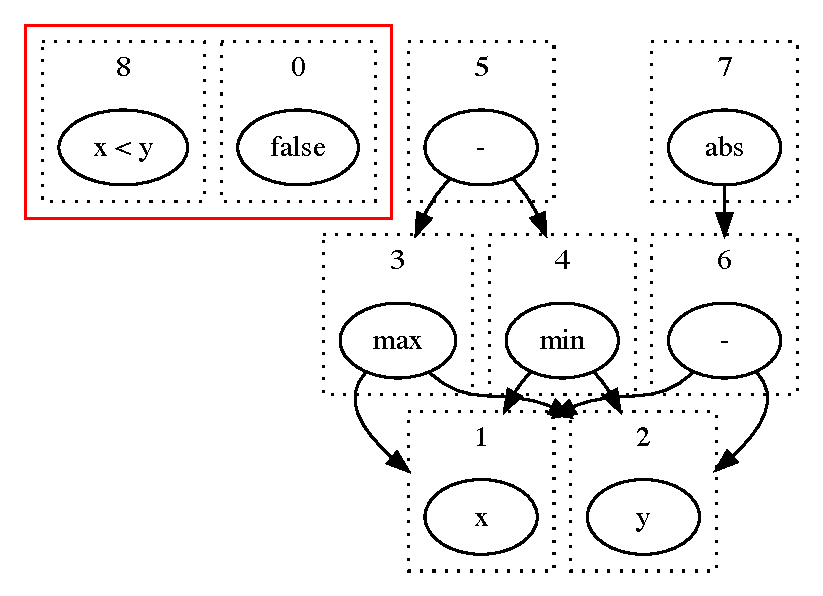
\includegraphics[width=4cm]{colors/gfx/example_graphs_res/00-init.pdf}
    }}
    \\
    {\small (2)}\newline
    merge$\lowerred$($[\tmax(x, y)]$, $[x]$)\newline
    merge$\lowerred$($[\tmin(x, y)]$, $[y]$)\newline
    merge$\lowerred$($[|x - y|]$, $[x - y]$)
    &
    \raisebox{-0.5\totalheight}{\fbox{
      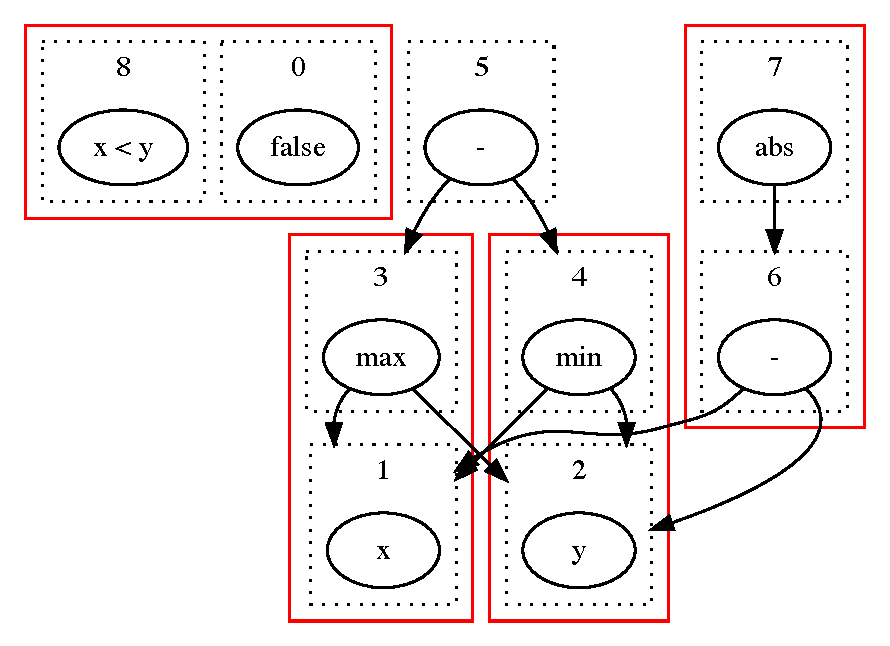
\includegraphics[width=4cm]{colors/gfx/example_graphs_res/01-after_rw.pdf}
    }}  
    \\
    {\small (3)}\newline
    rebuild$\lowerred$() \newline
    \quad $\downarrow$ \newline
    merge$\lowerred$($[x - y]$, \newline
    \hspace{3em} $\tmax(x) - \tmin(y)$)
    &
    \raisebox{-0.5\totalheight}{\fbox{
    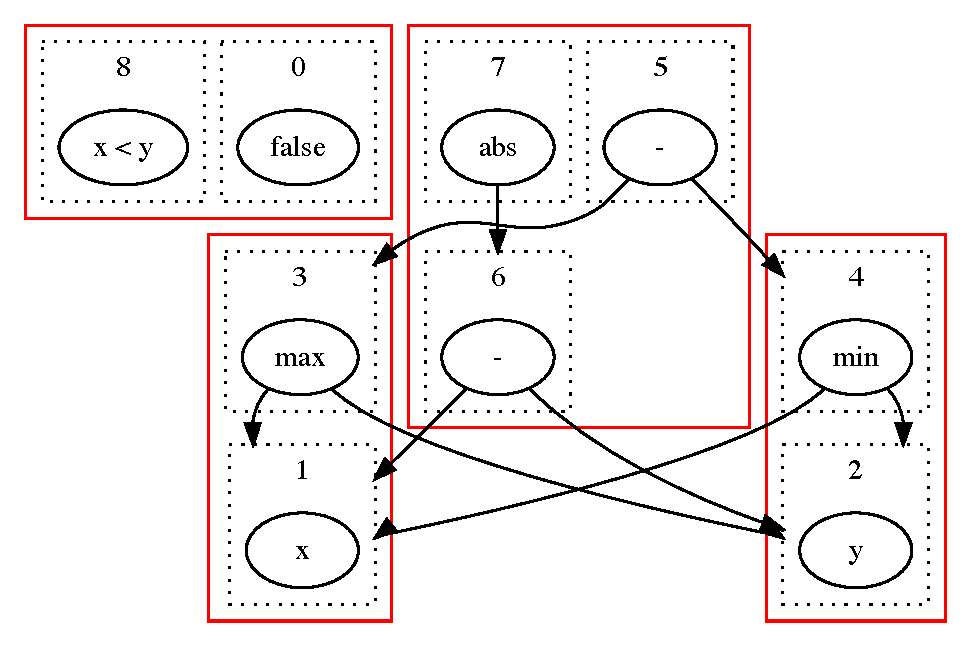
\includegraphics[width=4cm]{colors/gfx/example_graphs_res/02-final.pdf}
    }}

\end{tabular}
%    
\\
$\begin{array}{c}
        \mbox{rewrite rules} \\ \arrayrulecolor{gray!50!white}\hline
        {?x} < {?y} \Rightarrow \tmin({?x}, {?y}) \rwto {?x} \\
        \lnot{?x} < {?y} \Rightarrow \tmin({?x}, {?y}) \rwto {?y} \\
        {?x} < {?y} \Rightarrow \tmax({?x}, {?y}) \rwto {?y} \\
        \lnot{?x} < {?y} \Rightarrow \tmax({?x}, {?y}) \rwto {?x} \\
        {?x} < {?y} \Rightarrow |{?x} - {?y}| \rwto {?y} - {?x} \\
        \lnot{?x} < {?y} \Rightarrow |{?x} - {?y}| \rwto {?x} - {?y} \\
\end{array}$
\caption{\label{overview:colored:example}
    Rewriting with case-split in a colored e-graph.}

\end{center}
\end{figure*}

The semantics of a conditional rewrite rule in our domain is that the condition pattern should be matched and its root must be in the same e-class as $\ttrue$, and, additionally, the left-hand side should be matched as normal.
For simplicity of presentation, we pretend that $\lnot$ is a special case were the negated condition is e-matched and the e-class should contain $\tfalse$.

\smallskip
Starting with the base graph, \autoref{overview:egraph-max-min}(a), we describe the operation of Easter Egg
on the \cred color, corresponding to the case $\lnot x < y$.
The complement \cblue case ($x < y$) is analogous.

\begin{enumerate}[leftmargin=1.5em]
\item
    The value of $x < y$ is declared as $\tfalse$ via
    a colored merge.
    This yields a new \cred e-class.
\item
    Colored e-matching is performed against the premise of the c.r.r. $\lnot {?x} < {?y} \Rightarrow \tmax({?x}, {?y}) \rwto {?x}$.
    The condition of the rule, ${?x} < {?y}$, matches against the class $[x < y]$, 
    which is indeed in the same \cred e-class as $\tfalse$.
    
    Similar e-matches are carried out for the rules
    $\lnot {?x} < {?y} \Rightarrow \tmin({?x}, {?y}) \rwto {?y}$
    and
    $\lnot {?x} < {?y} \Rightarrow |{?x} - {?y}| \rwto {?x} - {?y}$.
\item
    The children of $\ecid3 - \ecid4 ~(\in M(\ecid5))$ are \cred-equivalent to those of $\ecid1 - \ecid2 ~(\in M(\ecid6))$, and,
    as a consequence, \cred congruence closure kicks in and performs a \cred union there.
\end{enumerate}

\medskip
The process for \cblue is analogous.
The case-split semantics is defined such that it records the fact
that \cblue and \cred are \emph{complements},
and as such extends $\equiv$ with the common equivalences,
$\congblue\cap\congred = \big\{\big\langle\ecid5,\ecid7\big\rangle, \ldots\big\}$.

\end{example}


\begin{comment}
   {\color{gray} 
\noindent\textbf{Colored insert.}~
As discussed, e-nodes should be shared, but until now no new e-nodes were added.
A simple example is the e-graph for the terms $1 + 2$, $2 + 1$ and $x$.
Now consider a new {\color{blue}blue} relation, and have the blue union $1 \congblue x$.
When we apply addition commutativity on this e-graph, a new e-node, ($1~+~x \rightarrow x~+~1$), should be added, but only for the blue layer.
In the current unoptimized approach, we share all e-nodes, so there will only be black e-nodes.
Meaning we will add the e-node to the original e-graph, but only unify the e-classes in the blue layer.
\ES{Should this be a theorem?} It is sound under the assumption that any e-node in the e-graph does not have any semantic meaning by itself.
For example, when encoding a problem to the colored e-graph, $sorted(l)$ has no semantic meaning unless $sorted(l) \cong true$ or $sorted(l) \cong false$.
And, If an additional e-node represented in the original e-graph does not affect the semantics, it is safe to add all colored conclusions as black e-nodes.


% Caveats and intro to optimizations section
To understand the weakness of this simple approach we should consider the setting of equality saturation.
A color will have additional unions, and therefore, might apply more rewrites resulting in additional e-nodes. 
The most basic approach of adding these e-nodes to the existing e-classes, hash-cons, and parents, is sound, but will result in additional e-matching results.
When considering the example from before, all colors can match on $x~+~1$.
A larger e-graph with more e-matches will lead to more rewrite rules being applied, and a slower rebuild process.
In addition, colored e-matching can find colored un-canonized matches.
Canonizing matches using the black congruence relation may lead to the addition of many unneeded e-nodes, as colored e-matching might produce duplicate matches.
But, canonizing using the colored congruence relation might produce different e-nodes for each color.
What makes matters more difficult, is that when all e-nodes are part of the original e-graph, they will not remain canonized by the colored relation, and might become "dangling" \ES{We will need to work on these explanations}.
}
\end{comment}
